%----------------------------------------------------------------

\begin{question}

Calcular, si existe, el siguiente limite
\[
        \lim_{(x,y)\to(0,0)} \cos\left({\frac{(x^2 + y^2)^{\frac{5}{2}}}{(x^2+2y^2)ln(1+x^2+y^2)}} \right)
    \]

\end{question}
%----------------------------------------------------------------
\begin{question}
   Sea la funcion $f:\Re^2\rightarrow\Re: f(x,y)=\sqrt{|x|^{\frac{8}{3}}|y|^{\frac{2}{3}}}$.
\begin{itemize}
    \item[a)] Analizar la continuidad de $f$ en $(0,0)$
     \item[b)] Probar que  $f_v(0,0)=\nabla f(0,0).v \quad \forall v \in \Re^2: ||v||=1.$
      \item[c)] Analizar la continuidad de $f_y $ en $(0,0)$
\end{itemize}
\end{question}

%---------------------------------------------------------------------
\begin{question}
    Aproximar, mediante un polinomio de grado adecuado, a
    \[
        e^{1 + \sin(0.1) + \cos\left(\frac{8}{9} \pi\right)}
    \]
\end{question}
%------------------------------------------------
\begin{question}
    Sea la función $f:\Re^2 \rightarrow \Re : f(x,y)=(x-1)^2 + (x-y)^4$. Hallar los puntos críticos de $f$ y clasificarlos como extremos locales, extremos absolutos o puntos silla, segun corresponda.
\end{question}
%------------------------------------------------------------------
\newpage

\begin{solution}
Para resolver el limite solicitado, en primer lugar se toma un calculo auxiliar, para analizar a qué tiende el argumento del coseno:
\[
        \lim_{(x,y)\to(0,0)} \frac{(x^2 + y^2)^{\frac{5}{2}}}{(x^2+2y^2)ln(1+x^2+y^2)} 
    \]
El cual se reescribe como
\[
        \lim_{(x,y)\to(0,0)} \frac{(x^2 + y^2)^{\frac{3}{2}}}{(x^2+2y^2)} .\frac{(x^2 + y^2)}{ln(1+x^2+y^2)} 
    \]
    Tomamos dos cálculos auxiliares para analizar cada término por separado, donde para resolver el término logarítmico, se busca utilizar los notables conocidos de funciones del tipo $f:\Re\Rightarrow\Re$

Primero se utiliza el límite notable conocido:    
\[
        \lim_{t\to 0} \
        \frac{ln(1+t)}{t}=1
    \]
    Llamamos  $t(x,y)=x^{2}+y^{2}$ y sabemos que 
   \[
        \lim_{(x,y)\to(0,0)} t(x,y)=0
    \]
    Definimos $g(z)=\frac{ln(1+z)}{z} $ y realizando la composición $f(x,y)=g\circ t(x,y) \hspace{0.25cm}\forall (x,y)\in \mathbb{R}^ 2 -(0,0)$ tenemos que
\[
        \lim_{(x,y)\to (0,0)} \
        g\circ t(x,y)=\lim_{(x,y)\to (0,0)} \
        g(t(x,y))=\lim_{t(x,y)\to 0} \
        \frac{ln(1+t(x,y))}{t(x,y)}=1
    \]
En segundo lugar, se analiza el termino restante 
auxiliar:
\[
        \lim_{(x,y)\to(0,0)} \frac{(x^2 + y^2)^{\frac{3}{2}}}{(x^2+2y^2)} 
    \]
Sabemos que
 \[
        0\le y^2+x^2\le x^2+2y^2    \Rightarrow   0\le \frac{1}{x^2+2y^2}\le \frac{1}{x^2+y^2} \Rightarrow   0\le \frac{(x^2 + y^2)^{\frac{3}{2}}}{x^2+2y^2}\le \frac{(x^2 + y^2)^{\frac{3}{2}}}{x^2+y^2}
    \]
Simplificando obtenemos que
 \[
         0\le \frac{(x^2 + y^2)^{\frac{3}{2}}}{x^2+2y^2}\le (x^2 + y^2)^{\frac{1}{2}}
    \]
Finalmente, por regla del sanwich obtenemos que:
\[
        \lim_{(x,y)\to(0,0)} \frac{(x^2 + y^2)^{\frac{3}{2}}}{(x^2+2y^2)}=0 
    \]
Por lo cual, 
\[
        \lim_{(x,y)\to(0,0)} \frac{(x^2 + y^2)^{\frac{5}{2}}}{(x^2+2y^2)ln(1+x^2+y^2)} =0
    \]
De esta manera, se calcula el limite solicitado:
    \[
        \lim_{(x,y)\to(0,0)} \cos\left({\frac{(x^2 + y^2)^{\frac{5}{2}}}{(x^2+2y^2)ln(1+x^2+y^2)}} \right)=1
    \]

\end{solution}
\newpage


\begin{solution}
\begin{itemize}
   \item[a)] En primer lugar, se nos pide analizar la continuidad de $f$ en el $(0,0)$. 
Sabemos que $f$ es continua en (0,0) si:  $\lim_{(x,y)\to(0,0)} \ f(x,y) = f(0,0)=0$. 
\[
        \lim_{(x,y)\to (0,0)} \sqrt{|x|^{\frac{8}{3}}|y|^{\frac{2}{3}}}=0=\sqrt{|0|^{\frac{8}{3}}|0|^{\frac{2}{3}}}=f(0,0)
    \]
 $\therefore\quad$ $f$ es continua en (0,0)

     \item[b)] En segundo lugar, se nos solicita probar que $f_v(0,0)=\nabla f(0,0).v \quad \forall v \in \Re^2: ||v||=1.$ 
Vamos a recordar que, si $f$ es diferenciable en (0,0) $\Rightarrow $ existen todas las derivadas direccionales y ademas $f_v(0,0)=\nabla f(0,0).v \quad \forall v \in \Re^2: ||v||=1.$ Demostraremos la diferenciabilidad de $f$ usando la definición formal 
\[
        \lim_{(x,y)\to (0,0)} \frac{\sqrt{|x|^{\frac{8}{3}}|y|^{\frac{2}{3}}}-0}{||(x-0,y-0)||}= \lim_{(x,y)\to (0,0)} \frac{|x|^{\frac{4}{3}}|y|^{\frac{1}{3}}}{||(x,y)||}= \lim_{(x,y)\to (0,0)} \frac{|x|}{||(x,y)||}.|x|^{\frac{1}{3}}.|y|^{\frac{1}{3}}=0
    \]
Sabemos que
\[
        0<x^2<x^2+y^2 \quad\backslash\quad  0<|x|<\sqrt{x^2+y^2} \quad\backslash\quad  0<\frac{|x|}{||x,y||}<1
    \]
Por lo cual, utilizando la propiedad de acotada por cero, sabemos que
\[
        \lim_{(x,y)\to (0,0)} \frac{|x|}{||(x,y)||}.|y|^{\frac{1}{3}}.|x|^{\frac{1}{3}}=0
    \]

De esta manera, sabemos que $f$ es diferenciable en $(0,0)$. Por lo cual, existen todas las derivadas direccionales en $(0,0)$ y ademas $f_v(0,0)=\nabla f(0,0).v \quad \forall v \in \Re^2: ||v||=1.$ 
      \item[c)] Finalmente, se pide analizar la continuidad de $f_y $ en $(0,0)$, donde lo calcularemos primero por definicion:
\[
         \lim_{y\to0} \frac{\sqrt{|0|^{\frac{8}{3}}|y|^{\frac{2}{3}}}-0}{y-0}=\lim_{y\to0} \frac{0}{y}=0
    \]
    Por lo cual:
    \[
     \partialy f(x,y)= \begin{cases}
            \;|x|^\frac{4}{3} .\frac{1}{3}.y^\frac{-2}{3}.sgn(y) \quad \text{Si (x,y) $\in \Re^2$ $\backslash$ $y\neq0$} \\[5pt]
            \;0\quad \text{Si $(x,y)=(0,0)$}\\[5pt] 
        \end{cases}
    \]
\end{itemize}
Sabemos que $f_y$ es continua en (0,0) si:  $\lim_{(x,y)\to(0,0)} \ f_y(x,y) = f_y(0,0)=0$, por lo cual el limite a analizar es: 
\[
        \lim_{(x,y)\to (0,0)} |x|^\frac{4}{3} .\frac{1}{3}.y^\frac{-2}{3}.sgn(y)
    \]
Para resolverlo, tomaremos la curva $\alpha(t)=(\sqrt{t},t) / \lim_{t\to0^+} \alpha(t) = (0,0)$
    \[
         \lim_{t\to0^*} \
          f\circ\alpha(t)=\lim_{t\to0^*} \
         \sqrt{t}^\frac{4}{3} .\frac{1}{3}.t^\frac{-2}{3}.sgn(t)=\frac{1}{3}\neq0
    \]
    Como el $\lim_{(x,y)\to(0,0)} \ f_y(x,y) \neq f_y(0,0)$, $f_y$ no es continua en (0,0).
\end{solution}
\newpage
\begin{solution}
     Se nos pide aproximar, mediante un polinomio de grado adecuado, a
    \[
        e^{1 + \sin(0.1) + \cos\left(\frac{8}{9} \pi\right)}
    \]
    Empezamos definiendo $f(x,y)=e^{1 + \sin(x) + \cos\left(y. \pi\right)}$
    dado que $f(x,y)$ es una composición de funciones  $C^\infty$, su desarrollo en serie de Taylor es válido.. Para conseguir una mejor aproximacion, se utiliza el polinomio de Taylor de orden 2, definido por:
     \[
        \pi_{f,(0,1),2}= f(0,1) + \nabla f(0,1)(x,y-1)  + \frac{1}{2}(x,y-1)\boldsymbol{H}_f(0,1)\begin{pmatrix}x\\y-1\end{pmatrix} \label{eq:polTay2}
    \]
    donde se centro el mismo en el punto $(0,1)$ ya que es el punto donde se pueden utilizar valores conocidos, a los solicitados por la consigna. 
    Primero, calculamos el gradiente de la funcion y luego lo evaluamos en el punto:
    \[
         \nabla f(x,y)=(e^{1 + \sin(x) + \cos\left(y. \pi\right)}.cos(x),e^{1 + \sin(x) + \cos\left(y. \pi\right)}.\pi.sen(y.\pi))  
    \]
     \[
         \nabla f(0,1)=(e^{1 + \sin(0) + \cos\left(1. \pi\right)}.cos(0),e^{1 + \sin(0) + \cos\left(1. \pi\right)}.\pi.sen(1.\pi)) =(1,0)
    \]
    Luego, calculamos la matriz Hessiana y de la misma manera, reemplazamos en el punto:
      \noindent 
    \begin{align*}
        \boldsymbol{H}_f(0,1) & =
        \left(\begin{array}{cc}
                      \displaystyle\partialx(e^{1 + \sin(x) + \cos\left(y. \pi\right)}.cos(x))            & \displaystyle\partialy (e^{1 + \sin(x) + \cos\left(y. \pi\right)}.cos(x))           \\[10pt]
                      \displaystyle\partialx  (e^{1 + \sin(x) + \cos\left(y. \pi\right)}.\pi.sen(y.\pi)) & \displaystyle\partialy (e^{1 + \sin(x) + \cos\left(y. \pi\right)}.\pi.sen(y.\pi))
                  \end{array}\right)\left.\rule{0pt}{1.1cm}\right\rvert_{(0,1)}             \\[2pt]
                              & =\left(\begin{array}{cc}
                                               \displaystyle e^{1 + \sin(x) + \cos\left(y. \pi\right)}.(cos^2(x)  -sen(x))              & \displaystyle -e^{1 + \sin(x) + \cos\left(y. \pi\right)}.cos(x).sen(y.\pi).\pi              \\[5pt]
                                               \displaystyle   -e^{1 + \sin(x) + \cos\left(y. \pi\right)}.cos(x).sen(y.\pi).\pi  & \displaystyle e^{1 + \sin(x) + \cos\left(y. \pi\right)}.(-sen^2(y.\pi).\pi^2-cos(y.\pi)\pi^2)
                                           \end{array}\right)\left.\rule{0pt}{0.7cm}\right\rvert_{(0,1)} \\[2pt]
                              & =\left(\begin{array}{cc}
                                               1    & 0    \\
                                               0 & \pi^2
                                           \end{array}\right)
    \end{align*}
    
Por lo cual, podemos reemplazar en el respectivo polinomio de Taylor:
 \[
        \pi_{f,(0,1),1}(x,y)= f(0,1) + \nabla f(0,1)(x,y-1)  + \frac{1}{2}(x,y-1)\left(\begin{array}{cc}
                                               1    & 0    \\
                                               0 & \pi^2
                                           \end{array}\right)\begin{pmatrix}x\\y-1\end{pmatrix} \label{eq:polTay2}
    \]
 Seguidamente, se evalua en los puntos pedidos
 \[
        \pi_{f,(0,1),1}(0.1,\frac{8}{9})= f(0,1) + \nabla f(0,1)(0.1,\frac{8}{9}-1)  + \frac{1}{2}(0.1,\frac{8}{9}-1)\left(\begin{array}{cc}
                                               1    & 0    \\
                                               0 & \pi^2
                                           \end{array}\right)\begin{pmatrix}0.1\\\frac{8}{9}-1\end{pmatrix} \label{eq:polTay2}
    \]
     \[
        \pi_{f,(0,1),1}(0.1,\frac{8}{9})\approx 1.165923
    \]
 Sabemos que, el polinomio de Taylor de una funcion, aproxima el valor de la misma en puntos que son cercanos a su centro, por lo cual concluimos que:

        \[
        e^{1 + \sin(0.1) + \cos\left(\frac{8}{9} \pi\right)}\approx 1.165923
    \]
    
\newpage
\end{solution}

\begin{solution}
    En el último ejercicio, se nos solicita hallar los puntos críticos de $f$ y clasificarlos como extremos locales, extremos absolutos o puntos silla, segun corresponda; siendo $f:\Re^2 \rightarrow \Re : f(x,y)=(x-1)^2 + (x-y)^4$. Sabemos que $xo$ es un punto crítico de $f$ si $f$ no es diferenciable en $xo$ o $\nabla f(xo)=0$, los mismos son posibles puntos donde $f$ puede tener un extremo.\newline
    Hallemos los puntos donde el gradiente de $f$ se anula:
     \[
     \nabla f(x,y)=( 2(x-1)+4(x-y)^3,-4(x-y)^3)
    \]
    \[
     \nabla f(x,y)=(0,0)\iff \begin{cases}
            \;2(x-1)+4(x-y)^3=0 \\[5pt]
            \;-4(x-y)^3=0
        \end{cases}
    \]
    Resolviendo el sistema de ecuaciónes, encontramos un único punto que anula ambas ecuaciones: $(x,y)=(1,1)$.\newline
    Seguidamente, para clasificar el punto critico, utilizaremos el criterio de la segunda derivada. Hallemos la matriz Hessiana de $f$:
      \noindent 
    \begin{align*}
        \boldsymbol{H}_f(1,1) & =
        \left(\begin{array}{cc}
                      \displaystyle\partialx(2(x-1)+4(x-y)^3)            & \displaystyle\partialy (2(x-1)+4(x-y)^3)           \\[10pt]
                      \displaystyle\partialx  (-4(x-y)^3) & \displaystyle\partialy (-4(x-y)^3)
                  \end{array}\right)\left.\rule{0pt}{1.1cm}\right\rvert_{(1,1)}             \\[2pt]
                              & =\left(\begin{array}{cc}
                                               \displaystyle 2 + 12(x-y)^2             & \displaystyle -12(x-y)^2              \\[5pt]
                                               \displaystyle   -4(x-y)^2  & \displaystyle 12(x-y)^2
                                           \end{array}\right)\left.\rule{0pt}{0.7cm}\right\rvert_{(1,1)} \\[2pt]
                              & =\left(\begin{array}{cc}
                                               2    & 0    \\
                                               0 & 0
                                           \end{array}\right)
    \end{align*}
    Ahora, se calcula el determinante de la misma para clasificar el punto:
        \noindent 
    \begin{align*}
        det(\boldsymbol{H_f(1,1))}
                              & =det\left(\begin{array}{cc}
                                               2    & 0    \\
                                               0 & 0
                                           \end{array}\right)=0 \Rightarrow  \text{El criterio no decide}
    \end{align*}
     Para lograr clasificar el punto de otra manera, vamos a analizar la funcion. Sabemos que $f(x,y)=(x-1)^2 + (x-y)^4 \geq 0$ por lo cual, los puntos donde se anula la función, son mínimos de la misma.
 \[
     (x-1)^2 + (x-y)^4 = 0\iff \begin{cases}
            \;x-1=0 \\[5pt]
            \;x-y=0
        \end{cases}
    \]
   Por lo tanto, el punto $(1,1)$ es un mínimo global de  $f$\newline
    $\therefore f$ tiene un solo punto crítico, en $(x,y)=(1,1)$ y el mismo es un mínimo de la funcion.
    Tambien, se puede ver de forma grafica
\begin{figure}[h!] % El entorno figure te permite incluir imágenes
    \centering
    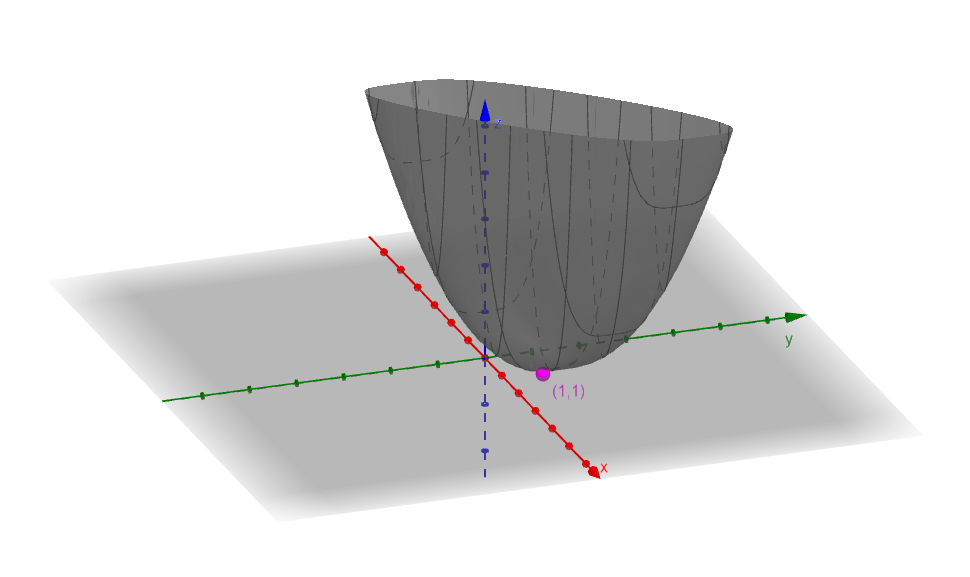
\includegraphics[width=0.5\textwidth]{Extremos20242c.png} % Cambia esta ruta por la ubicación de tu imagen
    \caption{Gráfica de $f$.}
    \label{fig:ejemplo} % Etiqueta para hacer referencia a la imagen
\end{figure}
\end{solution}
